\documentclass[10pt]{article}
\usepackage[margin=1in]{geometry}
\usepackage[parfill]{parskip}

\usepackage{amsfonts}
\usepackage{amsmath}
\usepackage{amssymb}
% \usepackage{mathtools}
\usepackage{graphicx}
\usepackage{tikz}
\usepackage{url}
\usepackage{color}
\usepackage{theorem}
% \usepackage{listings}
% \usepackage{savetrees}
% \usetikzlibrary{shapes}

\newenvironment{proof}{{\bf Proof:  }}{\hfill\rule{2mm}{2mm}}
\newenvironment{proofof}[1]{{\bf Proof of #1:  }}{\hfill\rule{2mm}{2mm}}
\newenvironment{proofofnobox}[1]{{\bf#1:  }}{}
\newenvironment{example}{{\bf Example:  }}{\hfill\rule{2mm}{2mm}}

\newtheorem{fact}{Fact}[section]
\newtheorem{lemma}[fact]{Lemma}
\newtheorem{theorem}[fact]{Theorem}
\newtheorem{definition}[fact]{Definition}
\newtheorem{corollary}[fact]{Corollary}
\newtheorem{proposition}[fact]{Proposition}
\newtheorem{claim}[fact]{Claim}
\newtheorem{exercise}[fact]{Exercise}

\linespread{1.5}
\setlength{\parindent}{0pt}
\setlength{\parskip}{1.9ex plus 0.5ex minus 0.2ex}

% Make title
\title{Partially Deamortized Packed-Memory Array}
\author{Michael A. Corley, Dhruv Matani, Gaurav Menghani, Deepak Nettem \\
        Department of Computer Science \\
        Stony Brook University \\
        Stony Brook, New York, 11794}
\date{}

\begin{document}
\maketitle
\bigskip

\clearpage

\section{Introduction}

One of the deficiencies in the traditional PMA is that one element
insertions might trigger a rebalance of the entire array, which costs
$\Theta(N)$ element moves. In contrast, the amortized number of
element moves, $\Theta(\log^2{N})$, is not that bad. When we do such
an insertion in a massive database, triggering a scan of the entire
database is infeasible. We may not be able to (or want to) wait while
the data structure rebuilds itself. To overcome this deficiency,
following the work(s) of Bender, Cole, Demaine, Farach-Colton, and
Zito \cite{2-simplified-algorithms}, and Willard \cite{willard},
Haodong Hu in his thesis \cite{haodong-thesis, adaptive-pma}
introduces a partially deamortized packed-memory array whose
insert/delete cost per update is at most
$\mathcal{O}({\sqrt{N}\log{N}})$.  Even though Haodong Hu's pardially
deamortized PMA is considerably simpler than the fully deamortized one
introduced by Willard, it is still hard to implement.

In the rest of this paper, we propose an algorithm to partially
deamortized the packed-memory that overcomes this deficiency making
for a practical implementation to be possible. Our partially
deamortized packed-memory array is a cache-oblivious data structure
that has a cost per insert of at most $\mathcal{O}(\sqrt{N})$ element
moves and $\mathcal{O}(1+ \frac{\sqrt{N}}{B})$ memory transfers, while having
the same performance of $\mathcal{O}(1+\frac{log^2{N}}{B})$ amortized memory
transfers as the traditional PMA.

We have also used the following referenced to learn about the Packed Memory, Deamortization, and related problems.

\begin{enumerate}
\item Eric Demaine's lecture notes \cite{demaine-lecture-notes}
\item Michael Bender's CSE638 lecture notes
\item Jeff Ericsson's Notes on deamortization \cite{jeffe-lecture-notes}
\end{enumerate}

\section{How to partially deamortize the PMA?}

We shall show how to partially deamortize a PMA (packed memory array)
only subject to inserts. Each operation will cost $O(\log^2{n})$
amortized and $O(\sqrt{n})$ worst case.

The general strategy that we shall adopt while trying to partially
deamortize the PMA is that of splitting the imaginary tree of the PMA
into a top half and a bottom half. The imaginary tree has height
$\log_2{n}$, so if we split it midway, we get roughly $1 +
\sqrt{n}$ imaginary trees, $\sqrt{n}$ of which correspond to actual
elements in the PMA. These trees are the $\sqrt{n}$ bottom trees, each
having a height of $\frac{\log_2{n}}{2}$.

We shall try to achieve the same amortized cost of $O(\log^2{n})$ per
element update, but we shall try to bring the worst-case cost per
update down from $O(n)$ to $O(\sqrt{n})$. This will come at the cost
of $O(n)$ extra space.

If a rebalance in the PMA causes elements to move within one of the
bottom trees, we perform such a rebalance normally since it doesn't
cost us more than $O(\sqrt{n})$. However, if a rebalance were to
affect one of the nodes in the top tree, it most certainly spans more
than one bottom tree. In such a situation, we re-build those trees
piece-by-piece. While the rebuilding process of these trees is in
progress, we shall perform element inserts into another data structure
called the \textit{parking lot}. \\

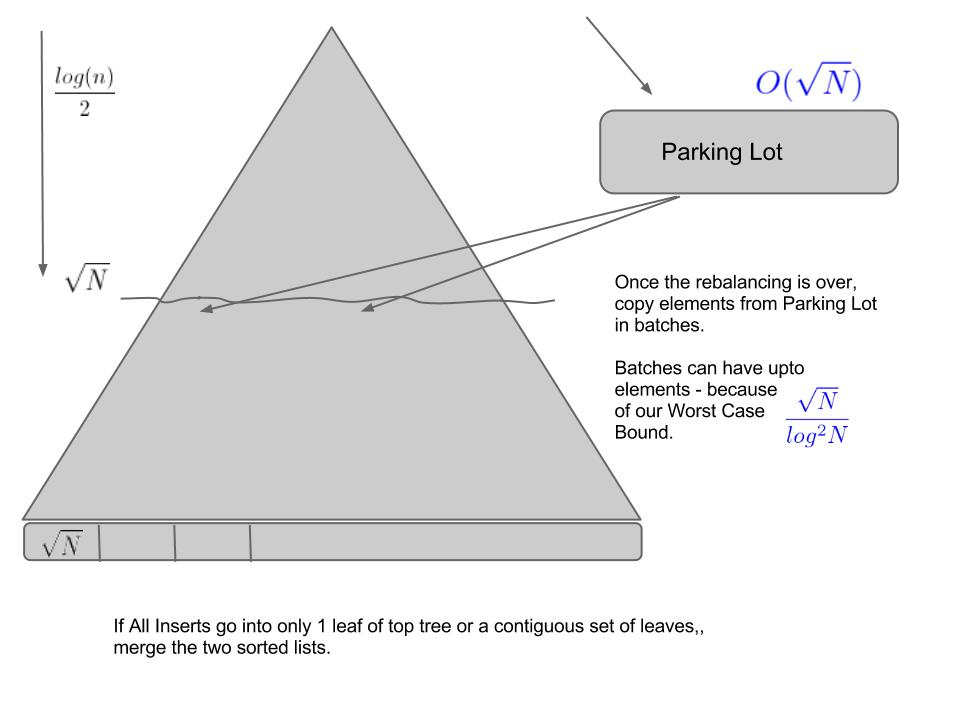
\includegraphics[width=120mm]{img1.jpg} \\


This \textit{parking lot} can be another PMA or even a simple array. 
The worst case cost to insert in the PMA or the array is
$O(\#\ of\ elements\ in\ the\ parking\ lot)$. We shall show that the
parking lot has size $O(\sqrt{n})$ and hence the worst case cost of
any insert into the parking lot is $O(\sqrt{n})$. We can not use a
linked list since we need to be able to do fast element lookups in the
\textit{parking lot}\footnote{Thanks to Pablo for pointing this out!}.

\begin{theorem}
\textbf{Rebuilding trees without knowing the tree span}

We can rebuild trees without known the span of the tree. i.e. without
knowing the number of elements that belong to the current imaginary
tree.
\end{theorem}

\begin{proof}
We assume that we need such a tool only to rebalance trees that are
rooted in the imaginary top tree, since the bottom trees can be
re-balanced normally.

We perform such a rebalance in 2 phases. In phase-1, we start copying
elements to a temporary array of size $O(\sqrt{n})$. We shall start
copying elements $\sqrt{n}$ at a time.

We know that we can choose any window in the PMA as long as the window
sizes grow exponentially (include reference - asked as an assignment
question, but Dr. Bender mentioned that there is a paper on
this). i.e. We select windows of size
$\sqrt{n},\ 2\sqrt{n},\ 4\sqrt{n},\ 8\sqrt{n},\ and\ so\ on\ldots{}$.

Once we have determined that a certain number of segments (say $c$) of
size $\sqrt{n}$ each is within threshold, we can start copying these
elements back to the PMA. The total amortized cost to perform such a
rebalance is $O(c\sqrt{n})$. The worst case cost per operation during
the whole rebalancing process is $O(\sqrt{n})$.

We note that we need to string together $c$ temporary arrays of size
$O(\sqrt{n})$ for this whole operation. Since $c$ is at most
$\sqrt{n}$, we need $O(n)$ extra space to perform the rebalance.
\end{proof}

\begin{theorem}
\textbf{The parking lot has $O(\sqrt{N})$ elements}

The number of elements in the parking lot never exceeds $O(\sqrt{n})$.
\end{theorem}

\begin{proof}

The parking will be most full when the root node of our imaginary tree
is rebalanced since that will trigger the rebuilding of $O(\sqrt{n})$
lower trees. When the root node is rebalanced, the parking lot will
contain $O(\sqrt{n})$ elements. We will show that the parking lot is
emptied before the root node is rebalanced again.

In the worst case, the number of elements in the PMA is just 1 less
than the maximum allowable for the given size. i.e. the PMA has
physical size $2n$, and currently has $n-1$ elements. So, the current density of the PMA is almost
$0.5$. Before the root node of the PMA is rebalanced, or a new PMA is triggered, it is possible to insert $O(\frac{n}{\log_2{n}})$ elements. This is by the standard PMA analysis.

We argue that $O(\sqrt{n})$ is smaller than  $O(\frac{n}{\log_2{n}})$, i.e the parking lot can be emptied before the root node is touched again.

Note that each of the leaves of size $\Theta(\log_2{n})$ can become completely full
since their density threshold is $1.0$.  Similarly, for the lower trees (of size $\sqrt{n}$ each), the
density threshold is roughly $0.75$. Hence, it has space for $0.25\sqrt{n}$
elements if we do not violate density thresholds. If we are okay with
violating density thresholds (as we shall see later), we can actually
insert $\frac{\sqrt{n}}{2}$ elements in each subtree of size
$\sqrt{n}$ and hence $\sqrt{n}$ elements in $k$ such subtrees. i.e. If
we want to insert $\sqrt{n}$ elements, we set $k = 2$. In our case, we
would want to insert $2\sqrt{n}$ elements to get $k = 4$. 

We consider multiple cases:

\begin{enumerate}

\item Suppose all the elements in the parking lot go to one of the
  ends (begin or end) of the PMA or to some specific part of the PMA
  (a.k.a. \textit{Hammer Inserts}). In this case, we can identify the
  $2\sqrt{n}$ lower trees that can be rebuilt and we use a simple
  merging strategy to offload the parking lot into these 2
  subtrees. The density thresholds for these subtrees is violated, but
  that is okay since the next rebuild will take care of that.

\item Suppose every element goes into a different subtree. In this
  case too, we pay a worst-case cost of $\Theta(\log^2{n})$ per insert
  (since we have just rebalanced the PMA), and we can actually perform
  batch inserts of $\Theta\left(\dfrac{\sqrt{n}}{\log^2{n}}\right)$ elements at a time to get a
  worst case running time of $O(\sqrt{n})$ per operation.

\end{enumerate}

In a similar fashion, we can sub-divide the inserts from the parking
lot into the PMA into cases where we insert $\Theta(\sqrt{n})$
elements into a lower tree or fewer and handle them separately. \\

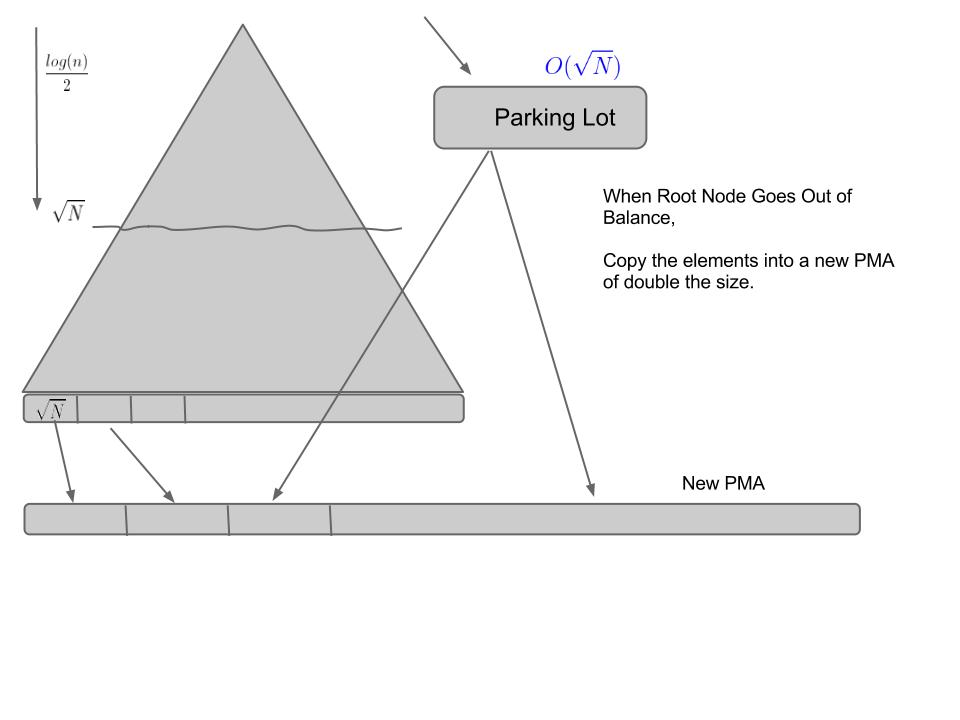
\includegraphics[width=120mm]{img2.jpg}

Additionally, if we detect that the sum of the sizes of the PMA and
the parking lot exceeds the density threshold at the root node, we can
start copying elements into a new PMA of twice the size. This
operation again copies $\sqrt{n}$ subtrees, each of size
$O(\sqrt{n})$. Since we do not insert elements into the PMA while it
is being rebalanced or copied, our parking lot is still capped at
$O(\sqrt{n})$ in size.

\end{proof}

\section{Querying the Partially Deamortized PMA}

Querying the \textit{PDPMA} is very simple. If no rebuild is in
progress, we query the PDPMA as we normally would. On the other hand,
if a rebuild is in progress, we query both the PDPMA as well as the
parking lot to answer queries. We are sure that the lower density
thresholds are met even during a rebuild since we are making the PMA
more sparse only if it has become too dense. i.e. we never violate the
lower density thresholds even while we are in the middle of a rebuild
operation.

\begin{thebibliography}{}

\bibitem{2-simplified-algorithms}
  Two Simplified Algorithms for Maintaining Order in a List, 
  Michael A. Bender, Richard Cole, Erik D. Demaine, Martin Farach-colton, Jack Zito, 
  2002

\bibitem{haodong-thesis}
  Cache-Oblivious Data Structures for Massive Data Sets,
  H. Hu,
  2007

\bibitem{adaptive-pma}
  An Adaptive Packed-Memory Array,
  M.A. Bender and H. Hu, 
  Transactions on Database Systems Special Issue on PODS '06, 32(4): 2007.

\bibitem{willard}
  A density control algorithm for doing insertions and deletions in a sequentially ordered file in good worst-case time, 
  D. E. Willard
  Information and Computation, 97(2):150–204, 1992.

\bibitem{demaine-lecture-notes}
  \url{http://courses.csail.mit.edu/6.851/spring12/lectures/L08.pdf}

\bibitem{jeffe-lecture-notes}
  \url{http://compgeom.cs.uiuc.edu/~jeffe/teaching/datastructures/notes/01-statictodynamic.pdf}

\end{thebibliography}

\end{document}
